\chapter{ Констукторский раздел}
\label{cha:design}
    В данном разделе будут рассмотрены схемы алгоритмов, требования к функциональности ПО, и определены способы тестирования.
    
    \section{Требования к функциональности ПО}
        В данной работе требуется обеспечить следующую функциональность.
        \begin{enumerate}
            \item Пользовательский режим:
            \begin{enumerate}
                \item возможность подать на вход две матрицы;
                \item вывод результата умножения трех алгоритмов.
            \end{enumerate}
	       \item Тестовый режим: 
            \begin{enumerate}
            	\item возможность проверки корректности работы алгоритмов.
            \end{enumerate}
            \item Экспериментальный режим: 
            \begin{enumerate}
                \item возможность замера процессорного времени работы алгоритмов для четного и нечетного размеров матриц.
            \end{enumerate}
        \end{enumerate}
	
	\section{Схемы алгоритмов}
        Ниже будут представлены схемы алгоритмов: \begin{enumerate}
            \item классическое умножение матриц (рисунок \ref{schema:ClassicMult});
            \item алгоритм Винограда (рисунок \ref{schema:Vinograd_1});
            \item алгоритм Винограда с оптимизацией (рисунок \ref{schema:Vinograd_Opt}).
        \end{enumerate}
      
       	    \begin{figure}[h!]
       		\centering
       		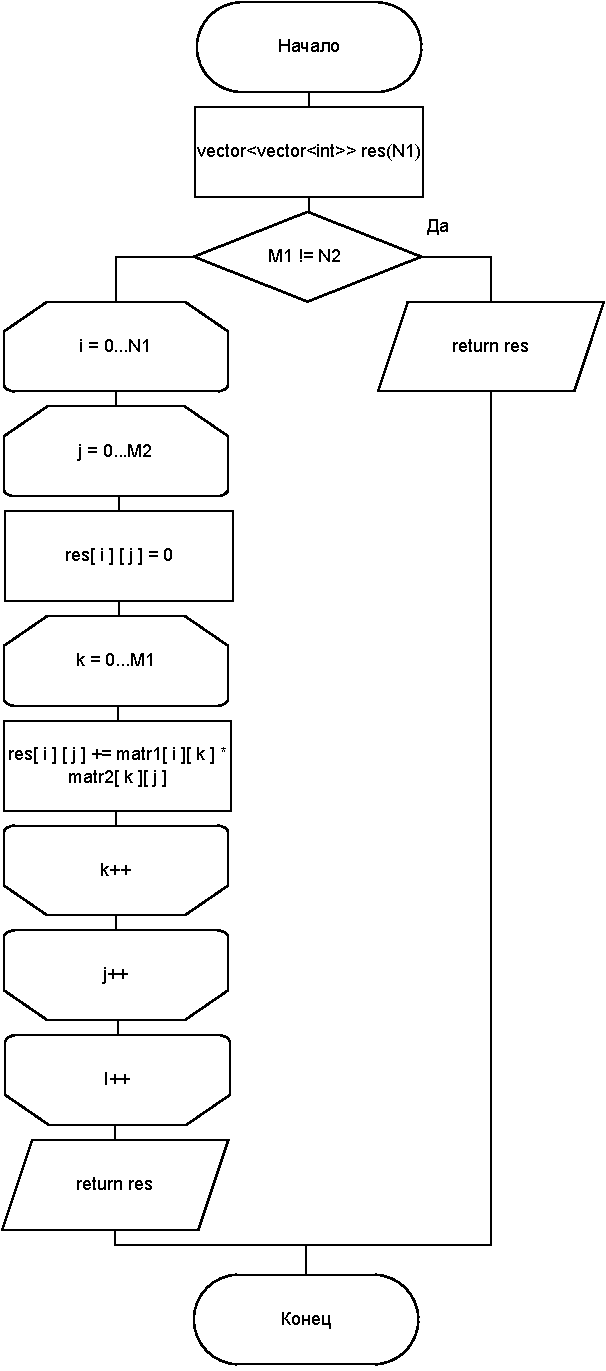
\includegraphics[scale=0.8]{ClassicMult.pdf}
       		\caption{Алгоритм классического умножения матриц}
       		\label{schema:ClassicMult}
       	\end{figure}\clearpage
       	
       	\begin{figure}[h!]
            \centering
            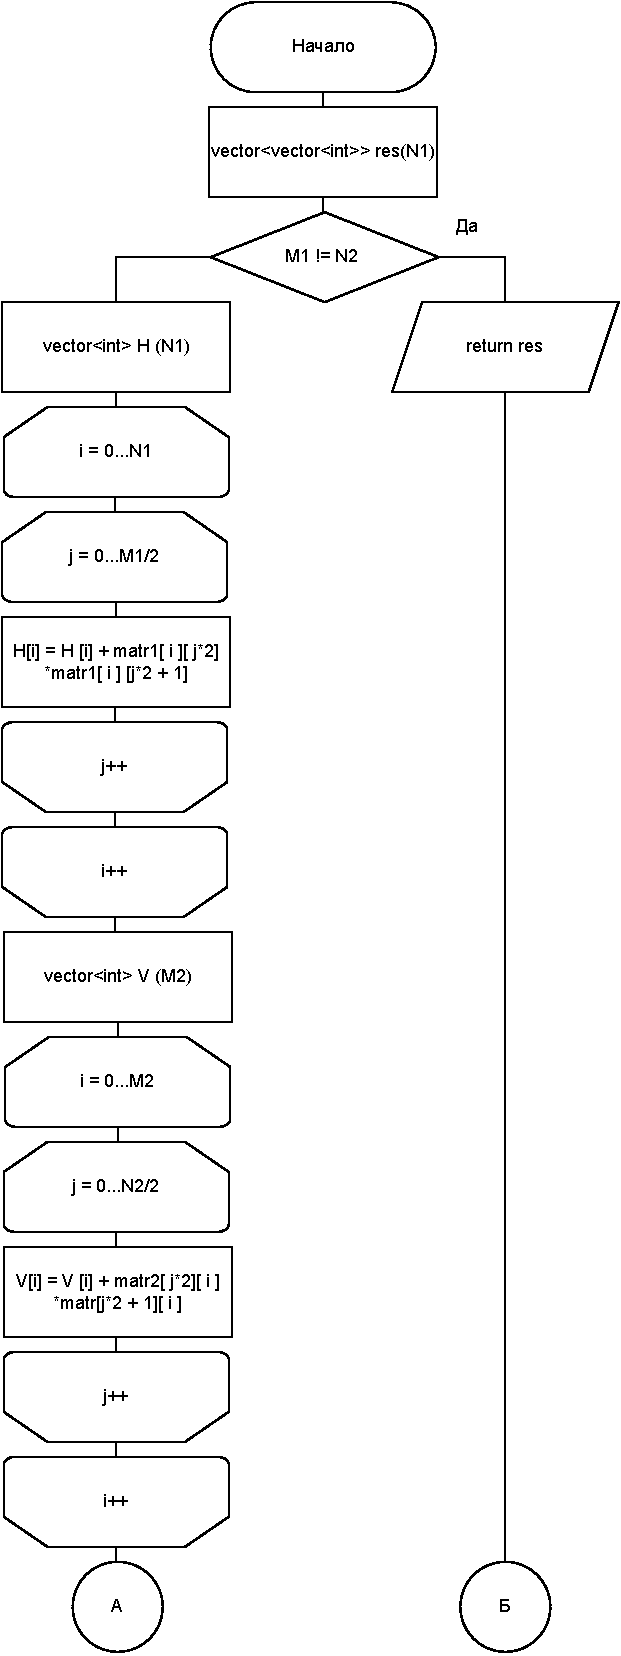
\includegraphics[scale=0.8]{Vinograd_1.pdf}
            \caption{Алгоритм Винограда без оптимизации Часть 1}
            \label{schema:Vinograd_1}
        \end{figure}\clearpage

        \begin{figure}[h!]
            \centering
            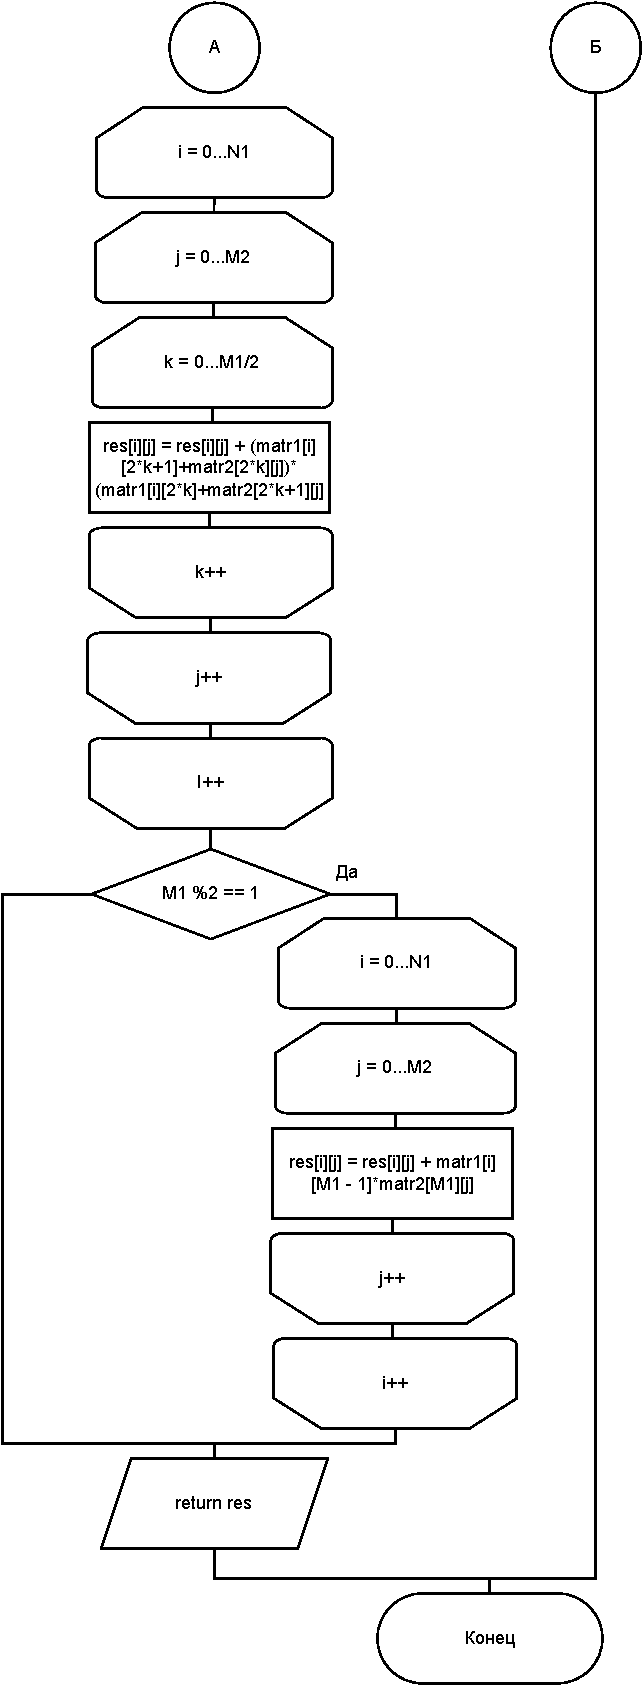
\includegraphics[scale=0.8]{Vinograd_2.pdf}
            \caption{Алгоритм Винограда без оптимизации Часть 2}
        \end{figure}\clearpage

        \begin{figure}[h!]
            \centering
            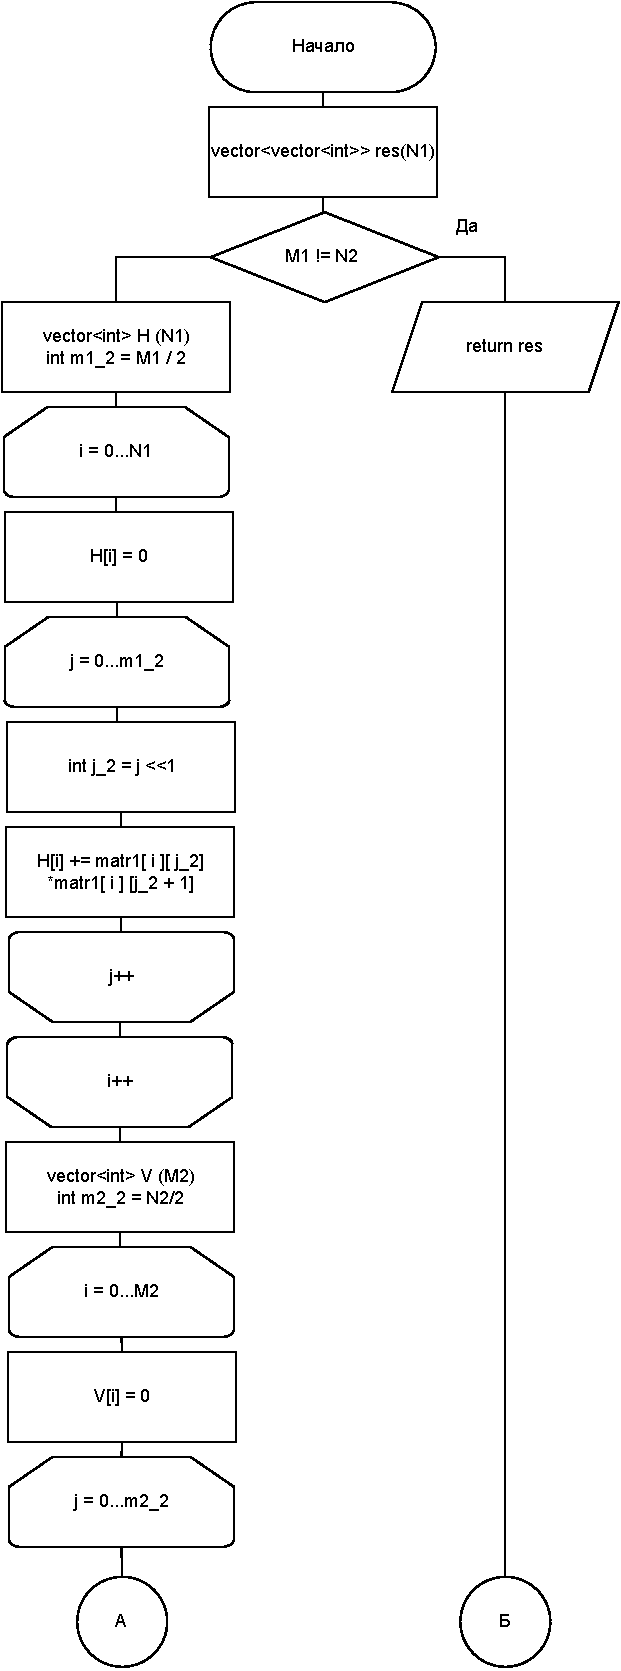
\includegraphics[scale=0.8]{VinogradOpt_1.pdf}
            \caption{Алгоритм Винограда с оптимизацией Часть 1}
            \label{schema:Vinograd_Opt}
        \end{figure}\clearpage

        \begin{figure}[h!]
            \centering
            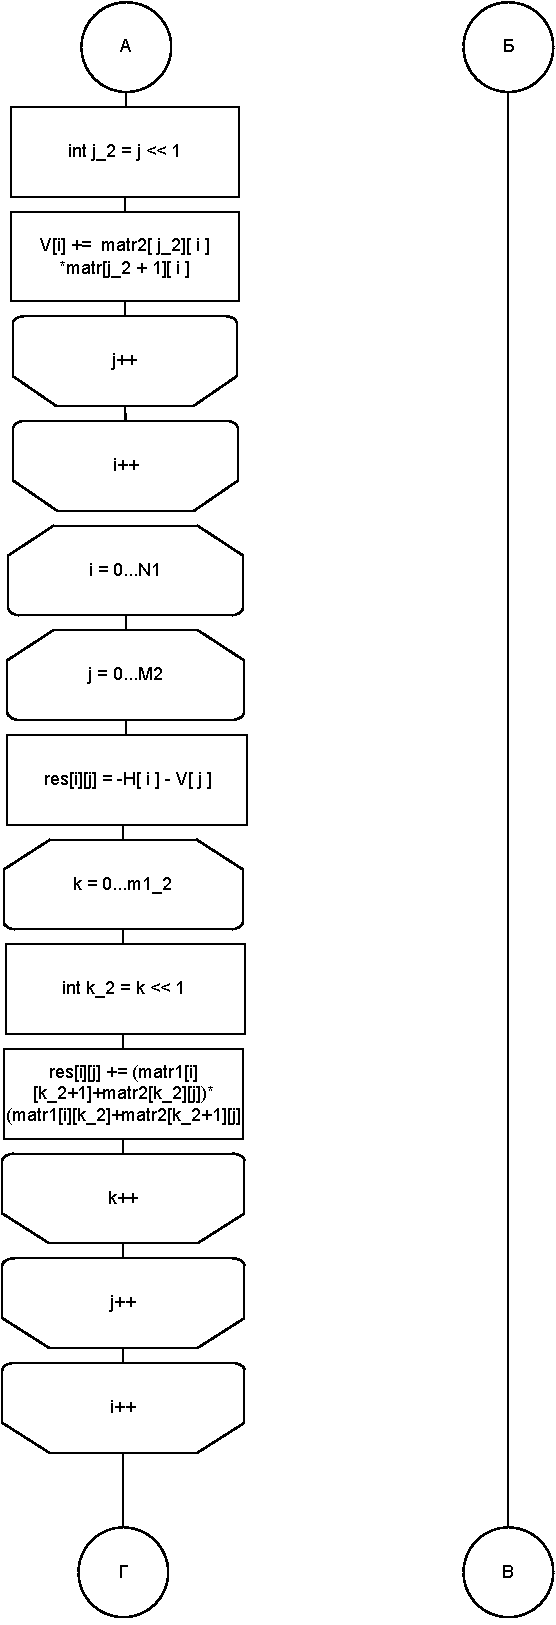
\includegraphics[scale=0.8]{VinogradOpt_2.pdf}
            \caption{Алгоритм Винограда с оптимизацией Часть 2}
        \end{figure}\clearpage

        \begin{figure}[h!]
            \centering
            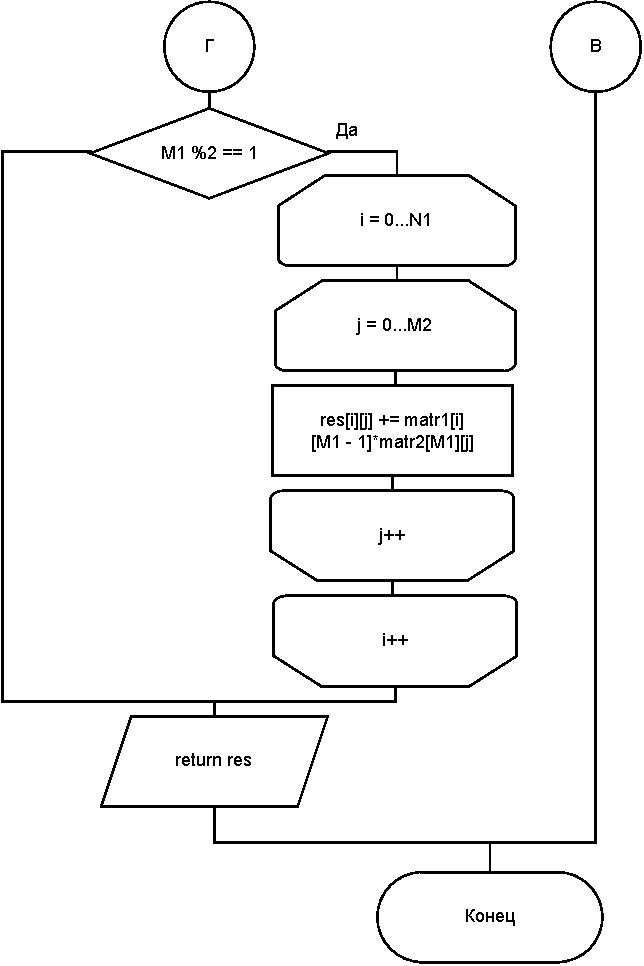
\includegraphics[scale=0.8]{VinogradOpt_3.pdf}
            \caption{Алгоритм Винограда с оптимизацией Часть 3}
        \end{figure}\clearpage
  	
    \section{Трудоемкость алгоритма}
    \par Трудоёмкость – количество работы, которую алгоритм затрачивает на обработку данных. Является функцией от длины входов алгоритма и позволяет оценить количество работы.
    \par Введём модель вычисления трудоёмкости.

    \subsection{Базовые операции}
    \par Стоимость представленных ниже операций единична:

    \begin{enumerate}
        \item \begin{math} =, +, +=, -, -=, *, *=, /, /=, ++, --, \% \end{math}
        \item \begin{math} <, \leqslant, >, \geqslant, ==, \neq \end{math}
        \item \begin{math} [ ] \end{math}
    \end{enumerate}

    \subsection{Условный оператор}

    \par \begin{math}if(\end{math} условие \begin{math}) \{\end{math}
    \par \begin{math} //\end{math} Тело А
    \par \begin{math}\}\end{math}
    \par \begin{math}else \{\end{math}
    \par \begin{math}//\end{math} Тело В
    \par \begin{math}\}\end{math}
    \par Пусть трудоемкость тела А равна \begin{math}f_A\end{math}, а тела В \begin{math}f_B\end{math}, тогда трудоемкость условного оператора можно найти по формуле (\ref{formula:IfTrud}):

    \begin{equation}\label{formula:IfTrud}
    f_{if} = f_{uslovie} + \begin{cases}
        min(f_A, f_B), &\text{-- лучший случай},\\
        max(f_A, f_B), &\text{-- худший случай}.\\
    \end{cases}
    \end{equation}

    \subsection{Цикл со счетчиком}

    \par \begin{math}for(int\end{math} \begin{math} i = 0; i < n; i++) \{\end{math}
    \par \begin{math} //\end{math} Тело цикла
    \par \begin{math}\}\end{math}

    \par Начальная инициализация цикла \begin{math}int\end{math} \begin{math}i = 0\end{math} выполняется один раз. Условие \begin{math}i < n\end{math} проверяется перед каждой итерацией цикла и при входе в цикл -- \begin{math}n + 1\end{math} операций. Тело цикла выполняется ровно \begin{math}n\end{math} раз. Счётчик \begin{math}i++\end{math} выполняется на каждой итерации, перед проверкой условия, т.е. \begin{math}n\end{math} раз. Тогда, если трудоёмкость тела цикла равна \begin{math}f\end{math}, трудоёмкость всего цикла определяется формулой (\ref{formula:ForTrud}):

    \begin{equation}\label{formula:ForTrud}
    f_{for} = 2 + n(2 + f) 
    \end{equation}

    \subsection{Классический алгоритм}

    \subsubsection*{Трудоемкость}
    \begin{equation}
    f_{FirstCycle} = 2 + N1 \cdot (2+ f_{SecondCycle})
    \end{equation}
    \begin{equation}
    f_{SecondCycle} = 2 + M2 \cdot (2 + f_{ThirdCycle} + 3)
    \end{equation}
    \begin{equation}
    f_{ThirdCycle} = 2 + N1 \cdot (2+ 8)
    \end{equation}
    \begin{equation}
    f_{ClassicMult} = 10 \cdot N1 \cdot M2 \cdot N1 + 7\cdot N1 \cdot M2 + 4 \cdot N1 + 2 \approx 10\cdot N1 \cdot M2 \cdot N1
    \end{equation}

    \subsection{Алгоритм Винограда}

    \subsubsection*{Трудоемкость}
    \begin{equation}
    f_{FirstCycle} = 2 + N1 \cdot (2+ \frac{M1}{2} \cdot (2 + 12)) = 7 \cdot N1 \cdot M1 + 2\cdot N1 + 2
    \end{equation}
    \begin{equation}
    f_{SecondCycle} = 7 \cdot N1 \cdot M2 + 2 \cdot N1 + 2
    \end{equation}
    \begin{equation}
    f_{ThirdCycle} = 2 + N1 \cdot (2+ M2 \cdot (2 + 7 + \frac{M1} {2} \cdot (2 + 23))) = 12 \cdot N1 \cdot M1 \cdot M2 + 9 \cdot N1 \cdot M2 + 2 \cdot N1 + 2
    \end{equation}
    \begin{equation}
    f_{if}= 2 + \begin{cases}
            0 &\text{-- лучший случай},\\
            15 \cdot N1 \cdot M2 + 2 \cdot N1 + 2 &\text{-- худший случай}.  
    \end{cases}
    \end{equation}
    \begin{equation}
    f_{Vinograd} = 12 \cdot N1 \cdot M1 \cdot N1 + 16\cdot N1 \cdot M2 + 7 \cdot M1 \cdot N1  + 6\cdot N1 + 6 + 
    \begin{cases}
            0 \\
            15 \cdot N1 \cdot M2 + 2 \cdot N1 + 2  
    \end{cases}
    \end{equation}

    \subsection{Оптимизированный алгоритм Винограда}

    \subsubsection*{Трудоемкость}
    \begin{equation}
    f_{FirstCycle} = 4 + N1 \cdot (2+ 1 + \frac{M1}{2} \cdot (2 + 10)) = 4 + 3\cdot N1 + 6\cdot N1 \cdot M1 
    \end{equation}
    \begin{equation}
    f_{SecondCycle} = 4 + M2 \cdot (2+ 1 + \frac{N2}{2} \cdot (2 + 10)) = 4 + 3\cdot M2 + 6\cdot M2 \cdot N2 
    \end{equation}
    \begin{equation}
    f_{ThirdCycle} = 2 + N1 \cdot (2+ M2 \cdot (2 + 7 + \frac{M1} {2} \cdot (2 + 18))) = 2 + 2 \cdot N1 + 9 \cdot N1 \cdot M2 + 10 \cdot N1 \cdot M2 \cdot M1
    \end{equation}
    \begin{equation}
    f_{if}= 2 + \begin{cases}
            0 &\text{-- лучший случай},\\
            13 \cdot N1 \cdot M2 + 2 \cdot N1 + 2 &\text{-- худший случай}.  
    \end{cases}
    \end{equation}
    \begin{equation}
    f_{Vinograd} = 5 \cdot N1 + N1 \cdot M2 \cdot( 9 + 10 \cdot M1) + 3\cdot M2 \cdot (1 + 2\cdot N2) + 6\cdot N1 \cdot M1 + 10 +
    \begin{cases}
            0 \\
            13 \cdot N1 \cdot M2 + 2 \cdot N1 + 2  
    \end{cases}
    \end{equation}

	\section*{Вывод}
    \par В данном разделе были рассмотрены схемы алгоритмов умножения матриц, введена модель оценки трудоемкости алгоритма, были расчитаны трудоемкости алгоритмов в соответсвии с этой моделью. При cхожем коэффициенте при старшем слагаемом в трудоемкости алгоритма Винограда и стандартного, доля долгих операций умножения в алгоритме Винограда меньше.
\newpage